\documentclass[../thesis]{subfiles}

\begin{document}
	\section{Results}
	\label{sec:cuda:results}

	\Cref{fig:cuda:results:times} shows the execution times achieved by this (naive) \cuda implementation. The superiority of the multicore implementation is clear, being around 30 times faster for $n=8000$. Yet, there are several reasons for this to happen.

	First, the multicore implementation has been the target of several optimizations in this document, while this is an initial completely functional \cuda implementation. Given the time already invested in the \intel\xeonphi coprocessor, it is not feasible to perform optimizations targeting the \cuda environment. Next, the absence of optimized \blas and \lapack packages suiting the needs of the implementation. \mkl provides it for both multicore environment and coprocessor, while manual (also naive) implementations had to be devised for \cuda. Lastly, the synchronization requirement between diagonals forces the runtime to return to the \cpu between two consecutive diagonals, creating a bottleneck when the amount of elements/blocks no longer provides enough parallelism to overcome the communication cost.

	\begin{figure}[htp]
		\begin{center}
			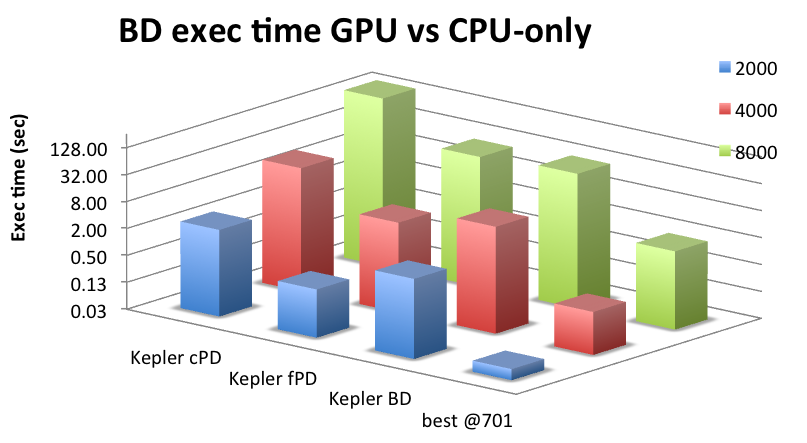
\includegraphics[width=0.9\textwidth]{assets/images/cuda/times.png}
		\end{center}
		\caption{Execution times for the CUDA implementation in a Tesla K20m (Kepler architecture).}
		\label{fig:cuda:results:times}
	\end{figure}
\end{document}

